\chapter{Overview of the Approach}

\section{Document management}

In the current thesis, we propose a client-based approach for the integration
open-source productivity software to enterprise document management systems. So
we discuss the case here when an enterprise company tries to replace the client
part of the document management system with an open-source alternative, while
keeping the existing proprietary server-side part of the system. As a
consequence, the center of our approach is the client -- the document management
part of the client, to be more exact (figure~\ref{fig:overview-architecture}).

\begin{figure}[H]
\centering
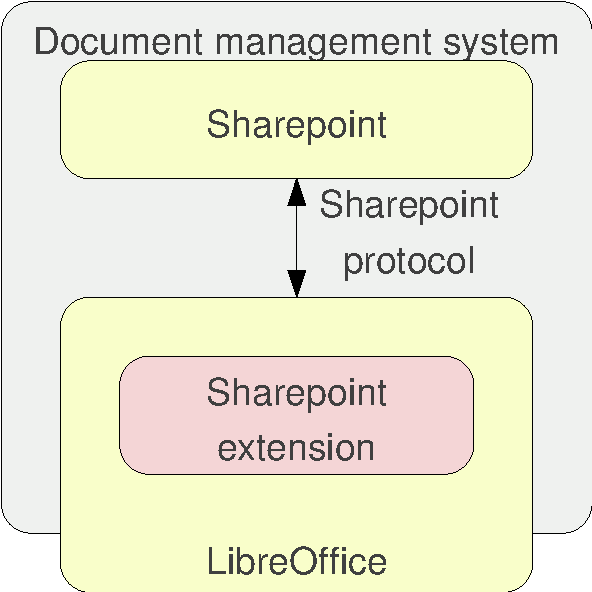
\includegraphics[width=250px,keepaspectratio]{overview-architecture.pdf}
\caption{Architecture of the approach}
\label{fig:overview-architecture}
\end{figure}

Components of the above example can be replaced, for example the Alfresco (with
its SharePoint module) can be used in place of SharePoint, and OpenOffice.org
can be used in place of LibreOffice. The SharePoint server, the office
productivity suite is already available.

By observing the network traffic between the SharePoint server and a native
Microsoft Office, the protocol can also be known. As mentioned earlier, the
documentation on its own is not enough, as it's not complete\footnote{And it's
purely a reference, there are no guide or tutorial to get started.}.

Finally at this stage the only remaining component is the SharePoint extension
in LibreOffice what is missing, and our approach creates that.

Note that Alfresco already has an OpenOffice.org extension called
OPAL\cite{opal}. That naturally uses Alfresco's native protocol to communicate
with the server. The following major changes are needed to make to suit our
needs:

\begin{itemize}
\item It's intended to be used with OpenOffice.org 3.1 -- the last stable
version of OpenOffice.org is 3.3, and it won't work with this version. The
oldest stable release of LibreOffice is based on OpenOffice.org 3.3 as well, so
poring the extension to 3.3 is essential to make it working at all with
LibreOffice.
\item It works by installing an additional module on the Alfresco server, so
the business logic is minimal in the extension. My approach is to communicate
without any server-side component installations required.
\item The SharePoint protocol supports more than Alfresco, the user interface
has to be extended to cover the new features.
\item Finally the used protocol has to be changed: by using the SharePoint
protocol, the extension can communicate with both SharePoint and Alfresco,
covering a lot from today's enterprise document management server
installations.
\end{itemize}

Now that we understood what component we want to create and from where, it's
essential to understand what workflow the document management clients take part
in (figure~\ref{fig:overview-workflow}).

\begin{figure}[H]
\centering
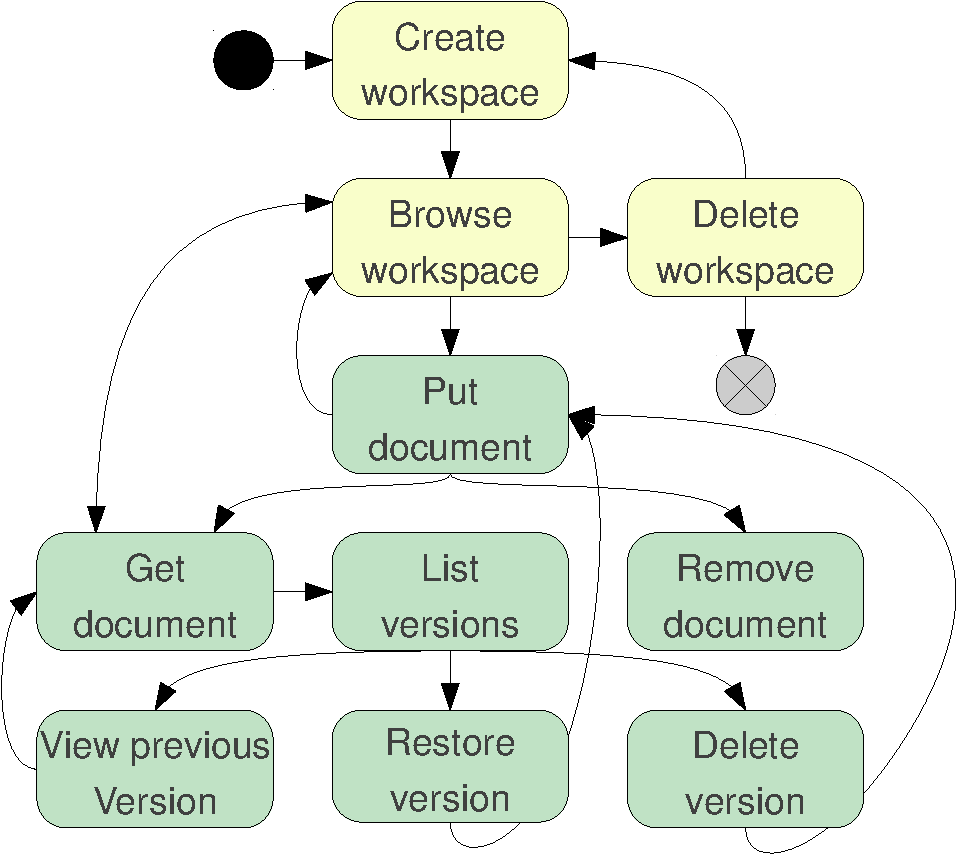
\includegraphics[width=300px,keepaspectratio]{overview-workflow.pdf}
\caption{Workflow of the approach}
\label{fig:overview-workflow}
\end{figure}

The workflow has the following steps:

\begin{itemize}
\item Create workspace: It creates a document workspace, which is the top-level
container for any document stored on the document management server.
\item Browse workspace: An existing workspace can be browsed, and a documents
can be put to workspaces.
\item Delete workspace: It's possible to get rid of no longer needed workspaces.
\item Put document: After selecting a target folder (using browse), a document
can be uploaded.
\item Get document: Existing documents can be downloaded for viewing or editing.
\item Remove document: Unneeded documents can be removed individually.
\item List versions: Every upload of a document may (depending on its type)
create a new version of the document. We can retrieve the list of this change log.
\item View previous version: older instances of a document can be viewed
read-only anytime.
\item Restore version: it's possible to revert all changes after a given
version with this step.
\item Delete version: older versions can be deleted.
\end{itemize}

\section{Workflows}

\subsection*{Document and workflow server decoupling}

Once the document-management client part of the system is in place, we propose
a decoupled approach to connect the document management system and the workflow
engine (figure~\ref{fig:decoupled-approach}). We already saw what are the
benefits of a system where each module can be replaced without altering the
whole system, the motivation is the same here.

\begin{figure}[H]
\centering
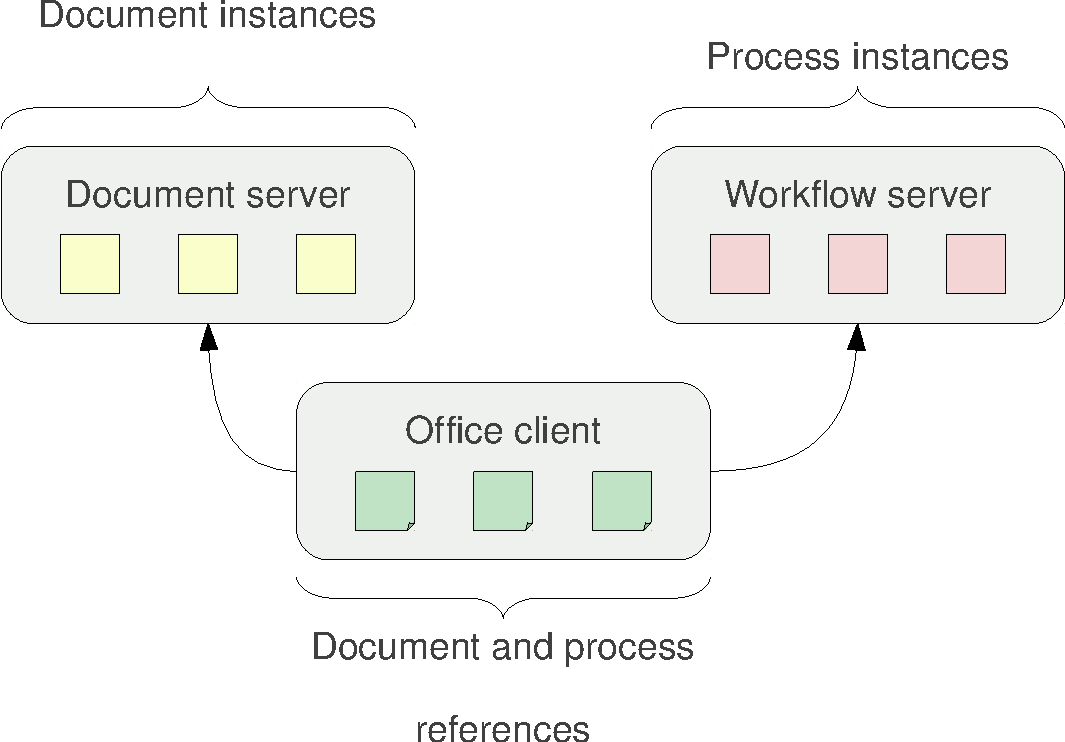
\includegraphics[width=300px,keepaspectratio]{decoupled-approach.pdf}
\caption{Architecture of the decoupled document based workflow approach}
\label{fig:decoupled-approach}
\end{figure}

In our proposal the \emph{document server and the workflow server is
decoupled}, and the connection between the two is provided by the office
client. Documents are stored on the document server, process instances are
managed by the workflow engine, and the client will have references to both.
Additionally, the workflow server will store references to documents, but such
references are resolved by the client. As a result, the workflow server will
not have to be altered in case the document server changes.

The system will have two operation modes:

\begin{itemize}
\item In case no workflow server is configured, or this is explicitly requested
by the user, the extension will still connect to the document server only.
\item Otherwise, the extension will query the tasks of the user in question
from the workflow server, and that will be the basis of all future work.
\end{itemize}

The possible states of the later operation mode is demonstrated on
figure~\ref{fig:decoupled-approach-workflow}.

\begin{figure}[H]
\centering
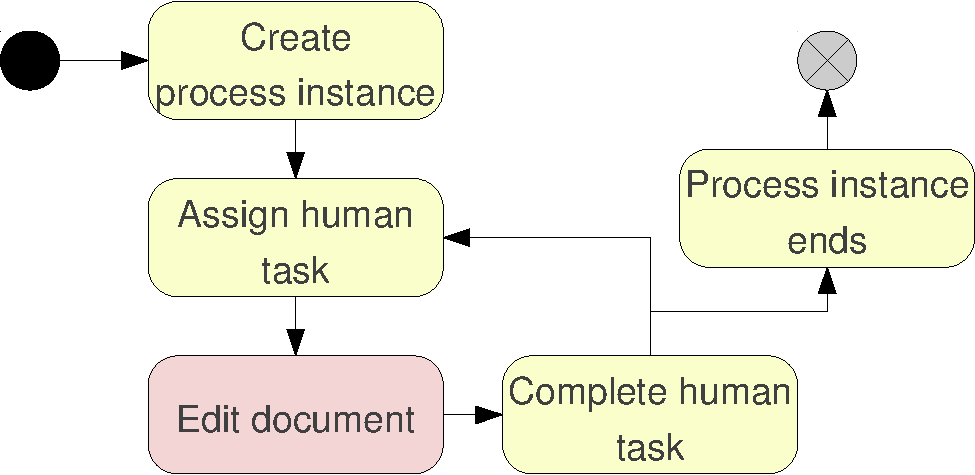
\includegraphics[width=300px,keepaspectratio]{decoupled-approach-workflow.pdf}
\caption{Control flow of the decoupled document based workflow approach}
\label{fig:decoupled-approach-workflow}
\end{figure}

The remaining part of this chapter describes each key feature we plan to design
later.

\subsection*{Starting process instances}

A process instance can be started externally or internally:

\begin{itemize}
\item If it is started externally, then the initiator of the process instance
connects to the workflow console server using the console UI or using some
other external application. After authentication, the user starts the process
instance by manually specifying the reference (URL) of the associated document.
\item A more integrated method is to start the workflow from the office client.
First the associated document has to be opened, then the office client can be
told to start a new process instance, once its type (a process definition) is
selected from the process definition list.
\end{itemize}

\subsection*{Incremental snapshots}

Once a process instance is started, its execution will be quickly blocked by
waiting for a human task to be executed. The simplest case is when this human
task is directly assigned to a user in the process definition. Given that each
process instance has an associated document, we can talk about assigned
documents. If a workflow server is configured, the file picker (the dialog that
shows up when the user wants to open or save documents) will list these
assigned documents for the user, providing them as documents in a virtual
folder.

\begin{figure}[H]
\centering
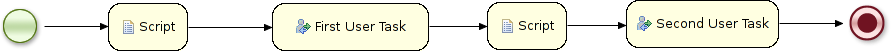
\includegraphics[width=350px,keepaspectratio]{step-bpmn.png}
\caption{Workflow with two statically assigned human tasks}
\label{fig:step-bpmn}
\end{figure}

Now in case the workflow has two human tasks and statically assigned users (see
figure~\ref{fig:step-bpmn}), the extension will offer completing the task when saving the
document. \emph{Incremental snapshots} is a feature that allows the user to
choose if the task completion is wished or not, so the document can be
incrementally saved to the document server as the task is being completed, and
once it is done, the task complete operation is performed on the workflow
server as well -- without leaving the office environment for a second.  Behind
the scenes, once the last human task is completed as well, the process instance
simply ends.

\subsection*{Group assignment}

A natural extension of naming the assigned users in the process definition is
think about roles or groups, so the exact user performing the task can be
determined later, at runtime. When the user reaches the file picker, a button
can navigate to an other virtual folder, called group tasks.

A new operation in this case will be \emph{claiming a task}, which means
selecting a document from the \emph{group tasks} folder and moving it to the
\emph{personal tasks} folder. Once the task is a personal one, the user can
proceed as before by editing the document, then completing the task.

The claim of a task can be undone: group tasks can be \emph{released} -- which
means moving from the \emph{group tasks} folder to the \emph{personal tasks}
one so other users can claim the task again.

\subsection*{Document masking}

Once the currently opened document has associated workflow information, the
editor can map parts of the document to parts of the process definition. Using
this knowledge, the editor can limit write access to the relevant subset of the
document, based on the current task instance associated to the document.

\subsection*{Decisions}

\begin{figure}[H]
\centering
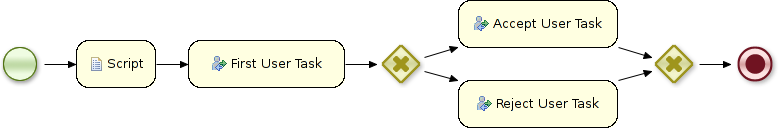
\includegraphics[width=350px,keepaspectratio]{decision-bpmn.png}
\caption{Workflow with a diverging and a converging gateway}
\label{fig:decision-bpmn}
\end{figure}

Figure~\ref{fig:decision-bpmn} shows a process definition containing a business
decision. The problem is that in this case the \emph{First User Task} can't be
completed without arguments: a decision has to be made to determine which
transition to fire after task completion.

The extension will query the list of possible choices from the workflow server
and the user will be able to make the decision when saving the document.

\subsection*{Audit log}

A benefit of using a workflow engine is the ability to query information about
completed process instances. The usual question are:

\begin{itemize}
\item When did an action happen?
\item Who performed the action?
\item Where did it happen?
\item What was the outcome of the action?
\end{itemize}

The extension will be able to show details of completed process, task and node
instances, answering these questions.

In this chapter, we shown what component of the document-based workflow system we
plan to implement. The next chapter will describe how the implementation is
designed to happen.
